\chapter{Background}

\section{Cattle Feed Efficiency}
To contextualise and drive the development of a framework for the development of phenotypic trait classifiers, the example phenotype of cattle feed effeciency was used. 

Feed effeciency in cattle is a phenotypic trait that is important for cattle manager. Conversion of feed to red meat in livestock is inherently inefficient in terms of feed intake to weight gain. For beef, current estimates of the ratio of feed intake to weight gain are between 5:1 and 10:1 \cite{Garnett2009}. Opportunities to improve this efficiency through genetic controls such as breed substitution, crossbreeding and genetic selection exist \cite{Hill2012} but data that shows how efficient individual animals are at converting feed to meat is essential in knowing which livestock to breed. This phenotype information can be used to extrapolate information about the genome which allows for the development of selection criteria for breeding objectives \cite{Pollak2012}.  

However, this specific livestock phenotype information is difficult to empirically obtain and there is currently a lack of data available. Current recording techniques have focused mainly on animals in feedlots, where the animals are kept in pens and fed \textit{ad libitum} at regulated times \cite{Arthur2005}.

This difficulty is compounded when considering livestock in pasture. Livestock in pasture feed directly from the pasture so it is not possible to regulate feeding times. Manually measuring feed intake of livestock in pasture is not practical as it would require significant manpower. Even in feedlots, where the process of measuring intake is easier because of the controlled way in which feeding is conducted, the cost of manpower is cited as the main reason for current lack of recording \cite{Barwick2010}. Furthermore, since heritability is both a property of the population and the environment \cite{Falconer1996}, measuring the traits of livestock in feedlots would not necessarily capture the traits of the same livestock in pasture. Attempts to capture this data through the use of chemical  markers to measure pasture intake in studies have had some success \cite{Barlow2009} \cite{Dove2006}; however, chemical markers have limitations and can only be used for short time periods. Therefore, to gain a robust understanding of the phenotype of individual animals, longer time periods of intake measurement are needed.

Opportunities exist in using devices to automate the collection of behavioural information however developing a practical measures of intake for livestock in pasture currently remains a serious challenge \cite{Cottle2013}. 

\section{Wireless Sensor Networks}
Wireless Sensor Networks are collections of small computers connected to sensors such as acceloremeter, magnetometer, audio etc. These small computers are named 'sensor nodes' and can perform processing on collected sensor data before communicating, typically over a radio connection, with other sensor nodes in the network. The sensors nodes are typically low power devices that can run in the field for extended periods of time. 

\subsection{Eartag Platform}

The Australian Commonwealth Scientific and Industrial Research Organisation (CSIRO) have previously developed sensor nodes that can non intrusively fit onto livestock and collect signal data including inertial measurement, Global Positioning System (GPS) measurement and audio data \cite{Guo2006}. As well as simply collecting signal data, these devices can also perform some processing on the data. There is a potential for these devices to be used for classifying livestock phenotypes such as feed efficiency.

For cattle, the CSIRO have developed a cattle eartag platform. A photo of the eartag is shown in figure \ref{eartag} and a photo of the eartag attached to a cow is shown in figure \ref{cow}.

\begin{figure}[ht!]
\centering
\begin{minipage}{.5\textwidth}
  \centering
  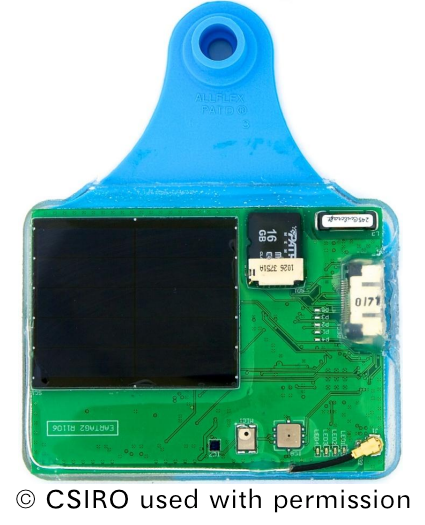
\includegraphics[width=0.4\textwidth]{images/eartag.png}
  \caption{Eartag}
  \label{eartag}
\end{minipage}%
\begin{minipage}{.5\textwidth}
  \centering
  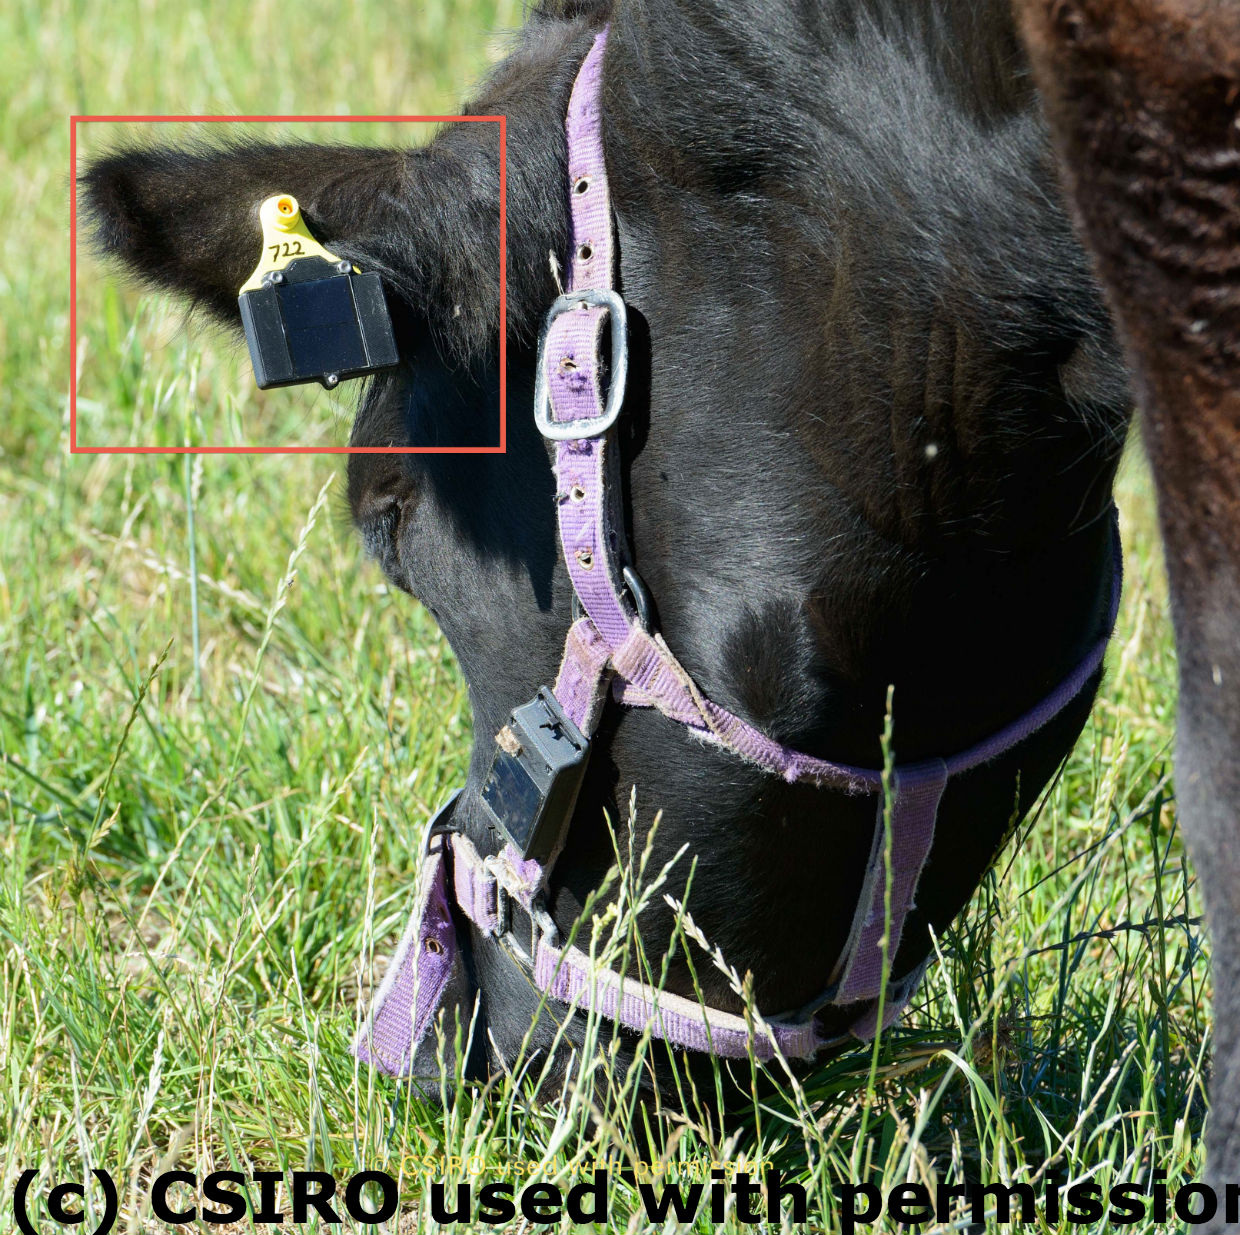
\includegraphics[width=.5\textwidth]{images/cow.jpg}
  \caption{Cow wearing eartag}
  \label{cow}
\end{minipage}
\end{figure}

The sensor node eartag platform is based on the 16 bit CC430F5137 microcontroller unit and has a range of sensors including audio, GPS, accelerometer, magnetometer and gyroscope.

\section{Classification algorithms}
In general, a classification algorithm takes some input and decides the class that that input should be categorised as \cite{someone}. For example, a classification algorithm could take five seconds of audio and categorise if there was human speech in the audio. 

In order to develop such a classification algorithm, a training set of data usually needs to be first constructed. This set of data contains example data that has been already classified (usually manually by a human) so that the algorithm can discover patterns and learn the rules needed to classify the data successfully \cite{someone}. This set of data is typically referred to as a \textit{training data set}. 

This learning phase is typically followed by a validation or testing phase. In order to measure the accuracy of an algorithm it is tested against previously manually classified example data that was not used in the learning phase. This example data is usually refered to as a \textit{test data set}. By testing the algorithm against data that was not used to train the algorithm, the robustness of the algorithm is tested. To further test the robustness of the algorithm there should also be large amounts of diversity between the example data in the test and training data sets.

This means that the steps to develop a classification algorithm is as follows:

\begin{enumerate}
\item Collect data

\item Annotate data into wanted categories

\item Split annotated data into training/testing sets

\item Develop classifier using training set

\item Test accuracy of classifier using testing set
\end{enumerate}

Developing a framework that could work with time series data collected from sensor nodes for the purpose of phenotype measurement would be useful. 
%maybe there'd be good resources about 'machine learning processes?'

\section{RESTful}
Representational state transfer (REST) is a way of architectually making data avaliable. The principle of REST is that data should be avaliable by reference rather than complete copy. This simplifies the process of sharing data. 

\section{HDF}
The Hierarchal Data Format (HDF) is a data format that is commonly used for storing large amounts of scientific data that will be written once, read often but not updated often. Is it commonly used for storing data from scientific experiments. 

\section{TDF}
The Tagged Data Format (TDF) is a data format developed by the CSIRO to store sensor data on SD storage.

\section{Python}
Python is a general use programming language. It is open source and there exist many libraries that can be used with it. In particular, there are many scientific libraries that simplify the process of working with large amounts of data. 

Python is a high level programming language that makes developing on it easy. For the most part, it has no significant performance compared to low level programming languages.

\subsection{matplotlib}
Matplotlib is a python library used for plotting data. It includes functionality to allow interactive plotting displays to be built 

\subsection{scikit-learn}

\section{Supervised Machine Learning Classification algorithms}

Machine learning classification algorithms are used to make decisions based on presented data. For supervised algorithms, data of which the result is known (training data) is used to train a model. Once trained, a model can be presented with unseen data and will automatically decide which class the data falls in to. 

Two standard machine learning algorithms that are used for classification problems, the Support Vector Machine (SVM) and the Aritificial Neural Network (ANN) are discussed in more detail below. 

\subsection{Artificial Neural Networks}
\label{ANNAppendix}

The Artificial Neural Network (ANN) is a machine learning paradigm that attempts to simulate the neurons of the central nervous system of animals and humans. Neural networks in humans and animals are considerably more complicated than ANNs \cite{Graupe2013}; however ANNs attempt to model the way in which real neural networks process information. ANNs can be used for machine learning and pattern recognition, the basic goal is to find a classification result given input data. For example, for recognition of spoken words, the input could be speech audio data and the output could be a number of different words (classes). For a certain speech input, one output word would be chosen. 

In an ANN, neurons are connected together to form a network. The way the neurons are connected is determined by the weight of their connections and this is the basis of the ANN. The weight of connection determines, for each neuron, how important the output of other neurons is. The larger the weight, the more important the connection. Weights can also be negative, which can be thought of as an inhibitive signal \cite{Graupe2013}.

A single neuron may receive inputs from many other neurons. Each input to the neuron is multiplied by the weight of the connection between the receiving and sending neuron. The receiving neuron then computes some mathematical function to determine whether, from the inputs it received, it will activate and send a signal forward. This continues until an output neuron activates which determines which output corresponds to the input given. 

Neurons are typically arranged in layers with only feed-forward connections \cite{Kuan}. The input to the ANN is given to the input layer, which then feeds forward to any number of hidden layers before progressing to an output layer where a classification is made. An example arrangement of neurons can be seen in figure \ref{ANN}. 

\begin{figure}[ht!]
\begin{center}
\leavevmode
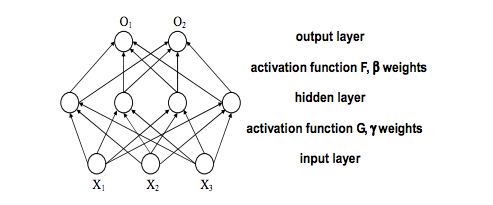
\includegraphics[width=0.5\textwidth]{images/ANN.png}
\end{center}
\caption[Example Artificial Neural Network]{An ANN with 3 input neurons, 4 hidden neurons and 2 output neurons. Figure from Kuan et al. \cite{Kuan}.}
\label{ANN}
\end{figure}

ANN are trained using supervised learning. That is, example input data is given to an ANN where the wanted classification result is known. Using a technique called back propagation, the ANN is progressively updated so that the error for classifying the example data is reduced.  


\subsection{Support Vector Machines}
\label{SVMAppendix}

Support Vector Machines (SVMs) are another machine learning supervised learning technique. Unlike the ANN which can classify input into multiple classes, the SVM only classifies input data into one of two classes. However, it is possible to build  multiple class classification systems using multiple SVMs. 

In training a SVM, the training data consists of input data and the correct binary classification (as there are only two classes that the input data can be classified into).  Using this training data, the SVM then finds the optimal hyperplane or set of hyperplane that best separates the input data of the two classes.  \cite{Jordan2008}

For a set of input data with n dimensions, a n-1 dimension hyperplane will be found. There can be many hyperplanes of this form but for SVMs the best hyperplane is often the hyperplane which maximises the margin between the two classes \cite{Jordan2008}. In this way, the classes are well defined and separated from each other. A simple, two dimensional example of the optimal hyperplane (simply a line in this case) can be seen in figure \ref{SVM}.

\begin{figure}[ht!]
\begin{center}
\leavevmode
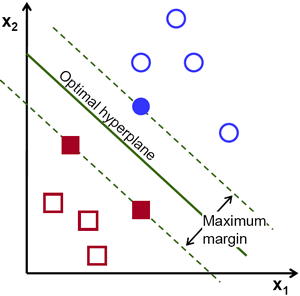
\includegraphics[width=0.5\textwidth]{images/svm.png}
\end{center}
\caption[Example Support Vector Machine]{The optimal hyperplane for a two dimensional example. The two classes are the red circles and blue squares. Figure from OpenCV \cite{SVM}.}
\label{SVM}
\end{figure}

Once trained, the SVM can accept input data and find on which side of the hyperplane the new input data lies. This allows the SVM to classify the data to a particular class. 
\section{Cow eartags}

